\documentclass[11pt,letterpaper]{article}
\usepackage[lmargin=1in,rmargin=1in,tmargin=1in,bmargin=1in]{geometry}
\usepackage{../style/homework}
\usepackage{../style/commands}
\setbool{quotetype}{true} % True: Side; False: Under
\setbool{hideans}{true} % Student: True; Instructor: False

% -------------------
% Content
% -------------------
\begin{document}

\homework{1: Due 09/28}{Clark Kent is Superman's critique on the whole human race.}{Bill, Kill Bill}

% Problem 1
\problem{10} Two relations, $F$ and $G$, are represented below. Are either $F$ or $G$ functions? Explain. 
	\[
	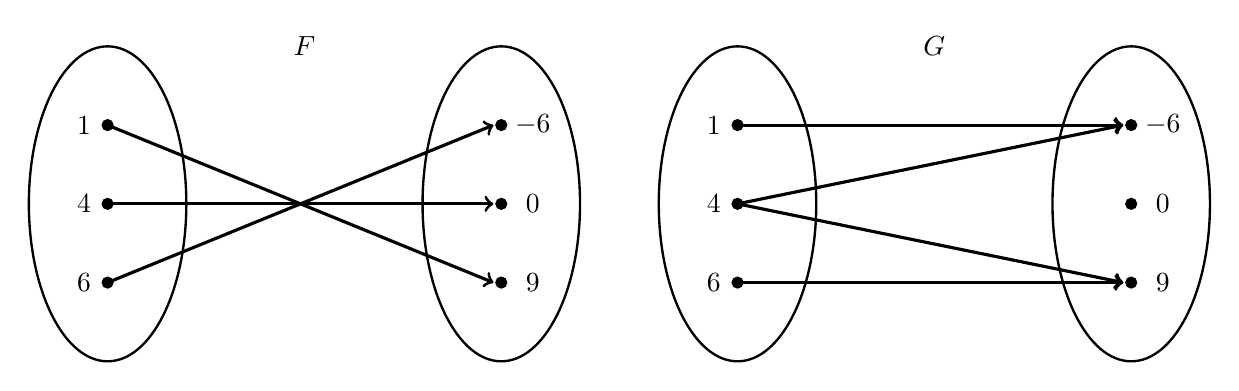
\begin{tikzpicture}
	\node at (2.5,2) {$F$};
	% Ellipses
	\draw[line width=0.03cm] (0,0) circle (1 and 2);
	\draw[line width=0.03cm] (5,0) circle (1 and 2);
	
	% Nodes
	\draw[fill=black] (0,1) circle (0.07);
	\draw[fill=black] (0,0) circle (0.07);
	\draw[fill=black] (0,-1) circle (0.07);
	
	\draw[fill=black] (5,1) circle (0.07);
	\draw[fill=black] (5,0) circle (0.07);
	\draw[fill=black] (5,-1) circle (0.07);
	
	% Arrow
	\draw[line width=0.04cm,->] (0,1) -- (4.9,-1);
	\draw[line width=0.04cm,->] (0,0) -- (4.9,0);
	\draw[line width=0.04cm,->] (0,-1) -- (4.9,1);
	
	% Labels
	\node at (-0.3,1) {$1$};
	\node at (-0.3,0) {$4$};
	\node at (-0.3,-1) {$6$};
	
	\node at (5.4,1) {$-6$};
	\node at (5.4,0) {$0$};
	\node at (5.4,-1) {$9$};
	
	\tikzset{shift={(8,0)}}
	%
	\node at (2.5,2) {$G$};
	% Ellipses
	\draw[line width=0.03cm] (0,0) circle (1 and 2);
	\draw[line width=0.03cm] (5,0) circle (1 and 2);
	
	% Nodes
	\draw[fill=black] (0,1) circle (0.07);
	\draw[fill=black] (0,0) circle (0.07);
	\draw[fill=black] (0,-1) circle (0.07);
	
	\draw[fill=black] (5,1) circle (0.07);
	\draw[fill=black] (5,0) circle (0.07);
	\draw[fill=black] (5,-1) circle (0.07);
	
	% Arrow
	\draw[line width=0.04cm,->] (0,1) -- (4.9,1);
	\draw[line width=0.04cm,->] (0,0) -- (4.9,1);
	\draw[line width=0.04cm,->] (0,0) -- (4.9,-1);
	\draw[line width=0.04cm,->] (0,-1) -- (4.9,-1);
	
	% Labels
	\node at (-0.3,1) {$1$};
	\node at (-0.3,0) {$4$};
	\node at (-0.3,-1) {$6$};
	
	\node at (5.4,1) {$-6$};
	\node at (5.4,0) {$0$};
	\node at (5.4,-1) {$9$};
	\end{tikzpicture}
	\]





\newpage





% Problem 2
\problem{10} Given the following tables, do $f(x)$ and $g(x)$ represent functions? Explain. 
	\begin{table}[!ht]
	\centering \setlength\arrayrulewidth{0.02cm}
	\begin{tabular}{c|ccc|c} 
	$x$ & $f(x)$ & \hspace{2cm} & $x$ & $g(x)$ \\ \cline{1-2} \cline{4-5}
	$1$ & $3$ && $1$ & $4$ \\
	$2$ & $6$ && $2$ & $1$ \\
	$3$ & $9$ && $3$ & $4$ \\
	$4$ & $2$ && $4$ & $5$ \\
	$5$ & $5$ && $1$ & $3$  
	\end{tabular}
	\end{table}
	


\vfill
\newpage



% Problem 3
\problem{10} Does the formula $f(x):= 2.31x + 9.55$ give a function? Explain. If it is a function, describe its graph. 




\vfill 



% Problem 4
\problem{10} For each of the following, indicate whether the equation is a linear equation (T), or not (F). 
	\begin{enumerate}[(a)]
	\item \uans{1.6cm}: $2x - 3y= 9$
	\item \uans{1.6cm}: $2x^2 + 5y^2= 7$
	\item \uans{1.6cm}: $x= 5$
	\item \uans{1.6cm}: $x= 6- y$
	\item \uans{1.6cm}: $y= x^2 + x + 1$
	\end{enumerate}



\vfill



% Problem 5
\problem{10} For each of the following, indicate whether the function is linear (T), or not (F). 
	\begin{enumerate}[(a)]
	\item \uans{1.6cm}: $y= 2x + 1$
	\item \uans{1.6cm}: $f(x)= 1 - 6x$
	\item \uans{1.6cm}: $y= x ( 2x + 1)$
	\item \uans{1.6cm}: $y= 2(x - 1)$
	\item \uans{1.6cm}: $f(x)= \frac{1}{3}x - 9$
	\end{enumerate}



\vfill
\newpage



% Problem 6
\problem{10} Given the data in the table below, is it reasonable to say that the data is linear? Explain. 
	\begin{table}[!ht]
	\centering
	\begin{tabular}{c|c}
	$x$ & $f(x)$ \\ \hline
	$1$ & $4$ \\
	$2$ & $6$ \\
	$3$ & $8$ \\
	$4$ & $10$ \\
	$6$ & $12$ 
	\end{tabular}
	\end{table}



\newpage



% Problem 7
\problem{10} Complete the following parts: 
\begin{enumerate}[(a)]
\item Find the equation of the line through the points $(1, -5)$ and $(-2, 13)$. \vfill
\item What is the slope and $y$-intercept of the line from (a)? \vfill
\item Sketch the line from (a) as accurately as possible. \vfill
\end{enumerate}



\newpage



% Problem 8
\problem{10} Consider the line given by $f(x)= 6x + 5$.
        \begin{enumerate}[(a)]
        \item Find the $y$-intercept for this line. \vfill
        \item Find the $x$-intercept for this line. \vfill
        \item Is the point $(0, 1)$ on the line? Explain. \vfill
        \item Is the point $(-1, -1)$ on the line? Explain. \vfill
        \end{enumerate}


\end{document}